%\documentclass[draft]{ws-procs11x85}
%\documentclass[square]{ws-procs11x85}
\documentclass{ws-procs11x85}
\usepackage{graphicx}

%\documentclass{article}

\begin{document}

\title{Understanding and Evaluating Medical Concept Embeddings}

\author{Andrew L. Beam$^*$, Inbar Fried, Nathan P. Palmer, Isaac S. Kohane}

\address{Department of Biomedical Informatics, Harvard Medical School,\\
Boston, MA, 02115, USA\\
$^*$E-mail: Andrew\_Beam@hms.harvard.edu\\
www.university\_name.edu}

\author{Benjamin Kompa}

\address{University of North Carolina, Chapel Hill,\\
Chapel Hill, NC, 27514, USA\\
E-mail: kompa@live.unc.edu}

\begin{abstract}
Word embeddings, also known as distributed representations, have seen rapid adoption in natural language processing (NLP) and machine learning. Though they are now standard practice in many areas of NLP and machine learning, they are just now begining to attract interest in biomedical and clinical informatics. In this article, we present an overview of the existing word embedding methodology and investigate their use for biomedical concepts. In addition, we propose a set of benchmarks so that researchers can evaulate concept embeddings and understand what aspects of the source data they capture. We provide the benchmarks and a set of reference embeddings as an R package to the community to encourage quick, easy, and reproducible comparisons of new embeddings in the future.
\end{abstract}

\keywords{Machine Learning; Distributed Representations; Word Vectors; Concept Embeddings; Unsupervised Learning}

\bodymatter


\section{Distributed Repsentations for Words and Concepts}\label{aba:intro}
The idea of a vectorized or distribution representation of a word has it roots in the neural language model of Bengio \cite{bengio2003neural}, though this model is actually a formalization of the ideas first put forth in [paper from the 50s]. However, it wasn't until the paper\cite{mikolov2013distributed} underpinning the wildly successful \emph{word2vec} software package which demonstrated that collapsing the neural language model of Bengio\cite{bengio2003neural} to a linear model enabled greater accuracy through training on much larger datasets that the idea of word embeddings finally came of age. Though they are often conflated, current distrubted representations are not an instance of deep learning, but are actually a speific kind of linear model, with explicit connections to many well known forms of matrix factorization.\cite{levy2014neural}



Word embeddings have ignited a furious amount of research after the the results of Mikolov\cite{mikolov2013distributed} et. al demonstrated that they are capable of capturing a surprising amount of semantic information. The central idea of a word embedding is to represent a word as a dense, real-valued vector that projects the word into $d$-dimensional space. Words that are similar in this space encode certain semantic and linguistic regularities from the source text. While classic NLP tasks, such as sentiment analysis and text classification, have been shown to benefit from distributed representations, what caused this approach to gain considerable attention was the observation that analogies could be solved using arithmetic vector operations. The now famous example of $man:woman::king:?$ can be sovled by the following operations on their corresponding word vectors: 
\begin{align*}
king - man + woman \approx queen
\end{align*}
Where the vector for $queen$ indicates a high cosine similarity to the vector resulting from $king - man + woman$. Thus, the analogy task is reduced to addition and subtraction on the word vectors.

 \subsection{Word2Vec and Glove}
The two most popular algorithms for computing word vectors to emerge from the last several years of work are \emph{word2vec}\cite{mikolov2013distributed} and \emph{Glove}\cite{pennington2014glove}. The ideas in \emph{word2vec} were originally presented in terms of two predictive models, the skip-gram and the CBOW. Thought the objective function as originally presented appeared somewhat mysterious, later it was shown that the skip-gram model with negative sampling was equivalent to factorizing a shifted pointwise mutual information matrix\cite{levy2014neural} for word-context pairs.

 \subsection{Medical Concept Embeddings}

\section{Benchmarks}
Here is where we will put the description of all of the benchmarks, put in \verb|\subsection{}| tags


\section{Results}
Here is where we will present the results for all of the different embeddings.
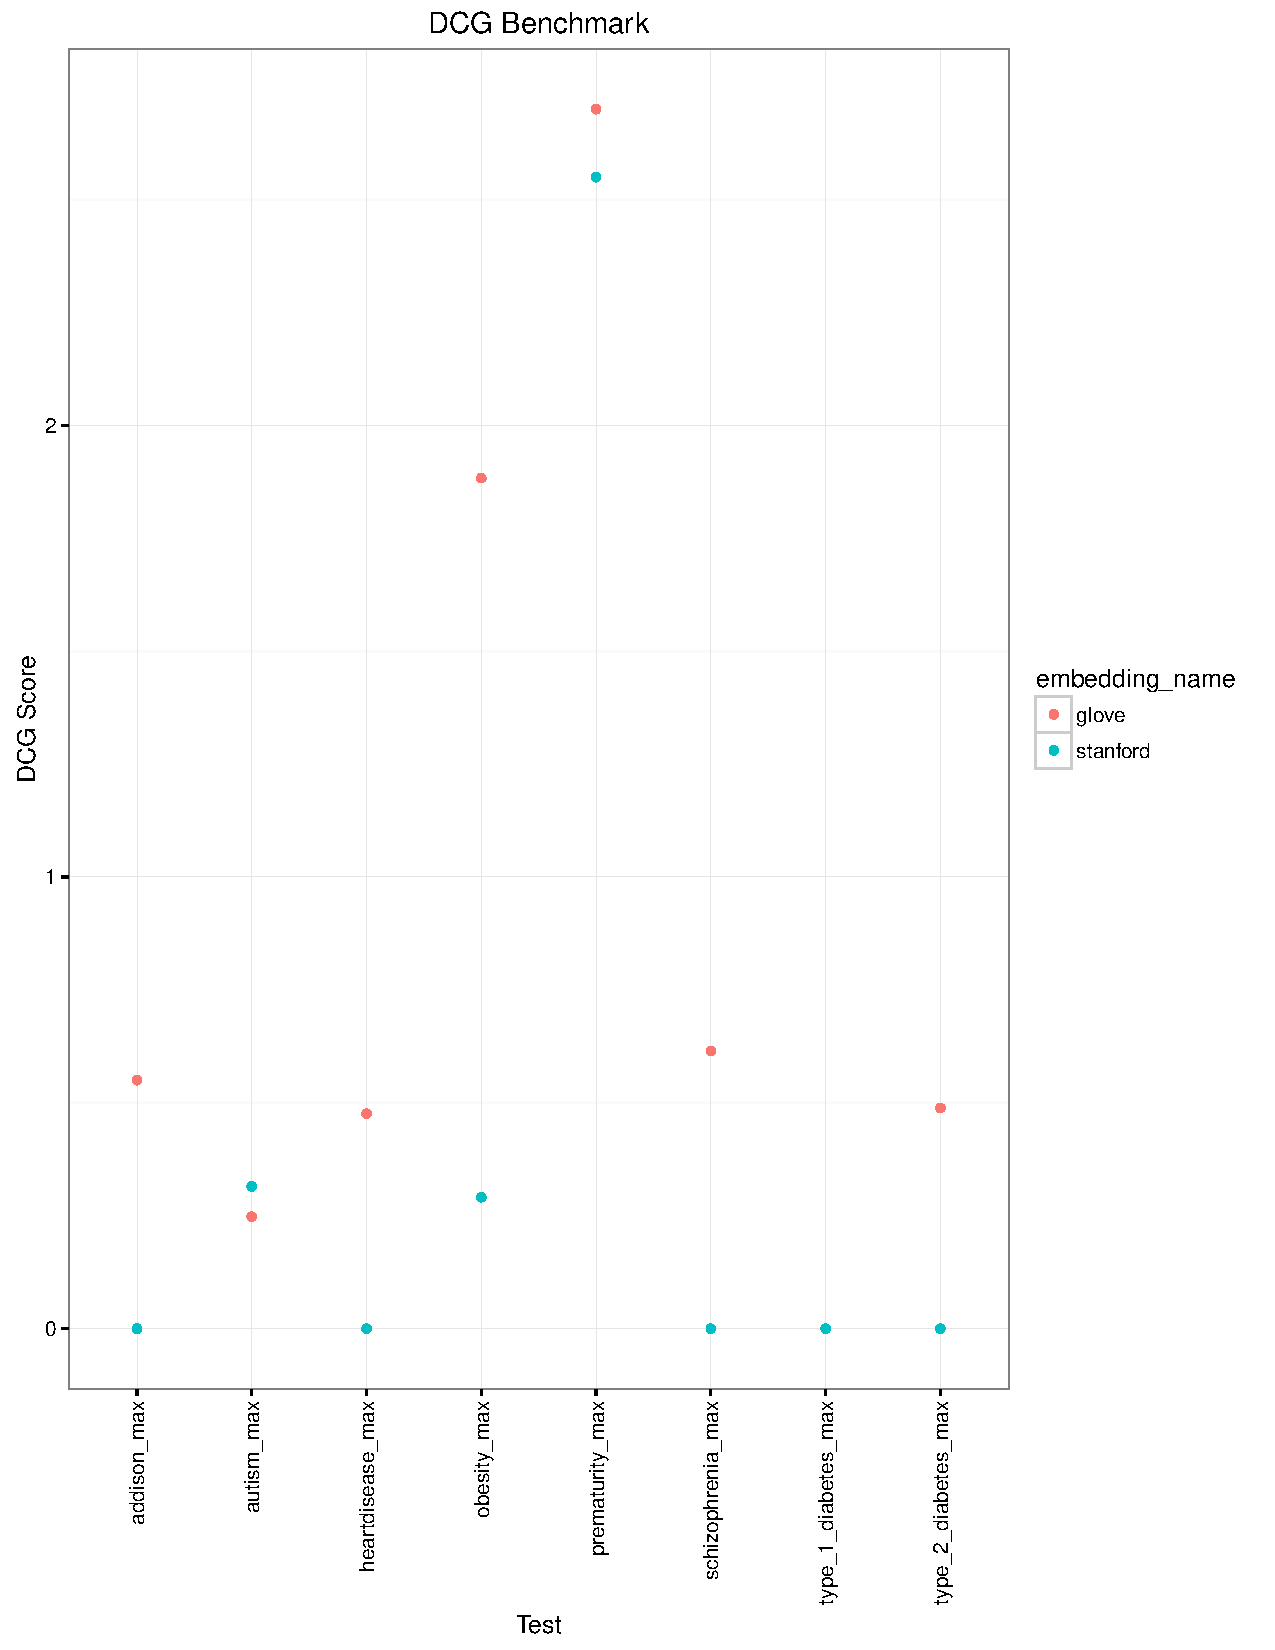
\includegraphics[scale=.5]{dcg_plot.pdf}

\bibliographystyle{ws-procs11x85}
\bibliography{ws-pro-sample}

\end{document}
